\documentclass[conference]{IEEEtran}
\IEEEoverridecommandlockouts
% The preceding line is only needed to identify funding in the first footnote. If that is unneeded, please comment it out.
\usepackage{cite}
\usepackage{amsmath,amssymb,amsfonts}
\usepackage{algorithmic}
\usepackage{graphicx}
\usepackage{textcomp}
\usepackage{xcolor}
\def\BibTeX{{\rm B\kern-.05em{\sc i\kern-.025em b}\kern-.08em
    T\kern-.1667em\lower.7ex\hbox{E}\kern-.125emX}}
\begin{document}

\title{Paper Title*\\
{\footnotesize \textsuperscript{*}}
\thanks{Identify applicable funding agency here. If none, delete this.}
}

\author{\IEEEauthorblockN{1\textsuperscript{st} Su,ZhaoLin}
\IEEEauthorblockA{\textit{dept. National Tsing Hua University,NTHU (of Aff.)} \\
\textit{name of organization (of Aff.)}\\
City, Country \\
email address}
\and
\IEEEauthorblockN{2\textsuperscript{nd} Given Name Surname}
\IEEEauthorblockA{\textit{dept. name of organization (of Aff.)} \\
\textit{name of organization (of Aff.)}\\
City, Country \\
email address}
\and
\IEEEauthorblockN{3\textsuperscript{rd} Given Name Surname}
\IEEEauthorblockA{\textit{dept. name of organization (of Aff.)} \\
\textit{name of organization (of Aff.)}\\
City, Country \\
email address}
\and
%\IEEEauthorblockN{4\textsuperscript{th} Given Name Surname}
%\IEEEauthorblockA{\textit{dept. name of organization (of Aff.)} \\
%\textit{name of organization (of Aff.)}\\
%City, Country \\
%email address}
%\and
%\IEEEauthorblockN{5\textsuperscript{th} Given Name Surname}
%\IEEEauthorblockA{\textit{dept. name of organization (of Aff.)} \\
%\textit{name of organization (of Aff.)}\\
%City, Country \\
%email address}
%\and
%\IEEEauthorblockN{6\textsuperscript{th} Given Name Surname}
%\IEEEauthorblockA{\textit{dept. name of organization (of Aff.)} \\
%\textit{name of organization (of Aff.)}\\
%vCity, Country \\
%email address}
}

\maketitle

\begin{abstract}
A concept of "cashier-free supermarket" is proposed in nowadays.
This is a work to use the Unity3D to simulate a complete supermarket.
 In our simulator scene,  we joined the item identification system.
It is including multi camera layout and weight sensor.
The item recognition is base on YOLOv3, and recognition processing by image which get form multi cameras.
From the simulator scene, it can be used in real supermarket.
This experiment can be used as a reference for the "cashier-free supermarket".


\end{abstract}

\begin{IEEEkeywords}

\end{IEEEkeywords}

\section{Introduction}
An increasing number of convenience stores as well as medium-scale and small-scale supermarkets appears in our surroundings.
To make a long-term profit, retailers desire to keep their overall cost as low as possible in terms of management, labor, logistics and properties.
According to the latest news, The Home Depot yearly labor cost 90,444 million, Costco yearly logistics cost 10,444 million.
Labor costs account for a large part of the operating costs of shopping malls.
So in recent years, many shopping malls have sought to transform and reduce labor costs with the same profits.
In recent year, there are many stores that require little or no manual labor, many stores have changed their business model..
They all use computer identification technology to reduce labor costs, and it has more advantages than traditional shopping malls.
They have quick checkout and self checkout technology, make people's shopping faster, make the management of operators more convenient.

Meanwhile, a concept of "cashier-free supermarket" is proposed in nowadays, which draws much public attention.
This technology is undoubtedly the best way to solve the labor cost at present, and over time it will gradually replace the traditional business model.
Now that the cashier-free supermarket has become a trend in the future development, so plenty of businesses has begun to join the ranks, and it will be a popular industries in the futures.
It is necessary to conform to the trend of development.
The number of unmanned supermarkets is increasing, and it is becoming an emerging business model in the future, for an instance,  the novel idea of ��Take it away��as announced by Amazon Go.
Amazon Go, Sam's Club Now and Taocafe are three pioneers that jump into the "cashier-free supermarket" technology and make it come true.
Amazon Go already started 5 unmanned stores in U.S. and they are planning to open up to 1000 stores till 2020.
Sensors and camera scan detect the categories and quantities of the products that a customer takes, it can make a preliminary settlement the self operation problems.
Moreover, with a proper camera layout, more integrated information can be gathered to strengthen our estimation of the quantitative variation of the products\cite{ERDEM2006156}.
Camera monitoring the purchasing behavior is an important part in a "cashier-free supermarket", and the change from a traditional supermarket to an advanced supermarket can be achieved by upgrading the capabilities and layouts of cameras, to provide an identification feature.
This paper will discuss the techniques of the modern cameras, mainly about device layouts, items category identification and quantity counting.
And achieve the establishment of Recognition System, the technology used and the problems solved.
%layout to cover all scene suitable




\section{Related Works}
\label{sec:rw}

Since the concept of "cashier-free supermarket" was put forward, it has attracted many people's attention.
It's a new style for shopping, and it is also a new solution which can show you another possibility in the future for command supermarket.
Saving costs and convenient management are its greatest feature.
In recent years, most of markets seeking transformation, this gave birth to examples such as Amazon Go and Sam's Club Now and Taocafe which are popular retailers in unmanned supermarket.
In the unmanned supermarket, all of them use the more advanced identification technology, plus their layout and the choice of camera equipment, realize the idea of "cashier-free supermarket".
For one of them, Amazon Go stores use a combination of sensors on the shelves, cameras and computer vision with machine learning.
Different from Amazon Go, Sam's Club pays more attention to camera layout aiming to plan shopping routes, and it use RFID\cite{1192765}.
Comparing the different retailers in our experiment, then build the camera layout first, then we combine the computer vision and sensor to identity the category and quantity of items.

\subsection{Multi Cameras System}

This is the foundation of "cashier-free supermarket".
It includes the choice of cameras, the number and placement of cameras in the scene, the angle and depth of field needed for visits.
In many shopping malls, the most commonly used camera layout is to place the camera on the top of the scene and on the shelves.
The rationality and feasibility of this layout are fully proved by \cite{1315006}.
In order to lower the overall cost of the sellers and economize resources, we aim to use the less cameras to cover whole scene while the clearest image can be obtained.
Through compare the camera layout of various supermarkets and chose one of the best-functioned layouts of cameras for our experiment, which use multi cameras and each camera is responsible for a specific area.
There are two type cameras which can be used in scene.
One is one-directional camera placed on the shelf, it requires high resolution in order to obtain high-definition pictures of items for identification.
Another is four-directional camera on the top of the scene, it is used to assist the camera on the shelf to recognize and observe the whole scene.
Next, we compare the cameras that are commonly used in the common market.
\textbf{BOSCH} FLEXIDOME IP panoramic 7000 MP, the camera is widely used in many shopping malls.
Different from the other cameras, it has the advantages of easy installation, wide viewing angle and fast transmission speed.
\textbf{AXIS} P3717-PLE is 4-directional cameras, it has reduced bandwidth and storage needs, 360�� IR illumination and remote zoom and focus and flexible positioning of four varifocal camera heads.
Getting all the information in this area and image obtained for each region are processed separately\cite{}, then we try to adjust the Field of View (FOV) aiming to ensure both, camera coverage maximizing and image clarity\cite{ERDEM2006156}.

\subsection{Computer vision}
At present, there are many kinds of architectures for computer vision, their slave processing methods and speed are different.
Two popular computer vision method are You Only Look Once (YOLO) and Regions with CNN features (RCNN)\cite{NIPS2015_5638}\cite{yolov3}.
They are base on CNN, both of them can use to computer vision and image processing, and they have strong recognition ability. Faster-RCNN is a command technology for researching feature map, and RPN network will complete the full operation of the map before send it to box regression layer and taxonomy\cite{NIPS2015_5638}.
It has the characteristics of fast and accurate identification of items.
YOLO just like its name "You Only Look Once", it has faster identification, which has developed to the third generation.
It is one of the most popular method in image processing area, and it is the first choice for some companies because it is open source and easy to build.
The YOLO input S*S grid, and every gird is responsible for the objects falling into it, then it can choose the maximal IOU of bounding box\cite{yolov3}.
Their comparison is shown in the Fig.1

\begin{figure}[htbp]
\centerline{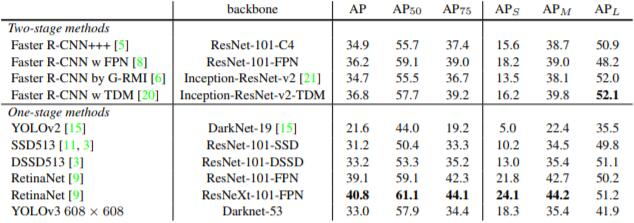
\includegraphics[width=8cm,scale=0.9]{YOLO-FRCNN.jpg}}
\caption{YOLOv3 is more suitable in state-of-the-art models.}
\label{fig}
\end{figure}

RCNN is often used in scenarios requiring more accurate recognition, a method for face detection\cite{7961803}\cite{Li_2015_CVPR}\cite{Yang_2016_CVPR}, to towards Real-Time object detection\cite{NIPS2015_5638}\cite{10.1007/978-3-319-10602-1_26}.
YOLO can also be used for accurate identification, it is based on the global information of the image to predict, and the error rate is low.
It can be used to interactive environments\cite{Gordon_2018_CVPR}, modeling behavior from visual data\cite{Ehsani_2018_CVPR}, anticipating visual representations from unlabeled video\cite{Vondrick_2016_CVPR}.
YOLO is more suitable than Faster-RCNN in our system by comparison.
YOLOv3 is chosen in our experiment since in processing medium-scale and small-scale supermarkets, it is based on Open Source Computer Vision Library(OpenCV) and Compute Unified Device Architecture(CUDA).
In the scene, it will put the images captured by the camera into YOLO for category judgment, and then output the results.

\subsection{Weight sensor}
In "cashier-free supermarket", weight sensor is used to identify the total weight of items, it support a measure about the number of items and assist the identify system.
Some supermarket already use the weight sensor, Amazon Go use the weight sensors as an assistant to determine the number of items on the shelves.

\subsection{official tones}

Amazon Go officials stressed that they could use computer vision, sensor fusion, and deep learning to make people shopping more convenient.
The store concept is considered as a revolutionary model which relies on the prevalence of smartphones and geofencing technology to streamline the customer experience, as well as supply chain and inventory management\cite{GREWAL20171} .
Electronic shelf label (ESL)


\subsection{end-user comments}

According to some end-user comments, the existence of trans-era science and technology changes our consumption pattern.
They think the traditional supermarkets need to be transformed, and it can improve the way of people's shopping.
Most of people think the new technology can give them a new way for shopping, and the new shopping mode will become the mainstream way of consumption, because it can reduce cost and save much time.
However, some people think it makes shopping a hassle since Amazon Go omitted the need for closing account by human, and it is hard for the aged to use smartphone, it incurring burden onto customers, and some people can not use the new technology, so the "cashier-free supermarket" promotion is still a problem.




\section{Method}

In this section, we will discuss the achievement of the "cashier-free supermarket", and the method what we use in our experiment.
The main parameters and the relationship between them are shown in the Fig.2

\begin{figure}[htbp]
\centerline{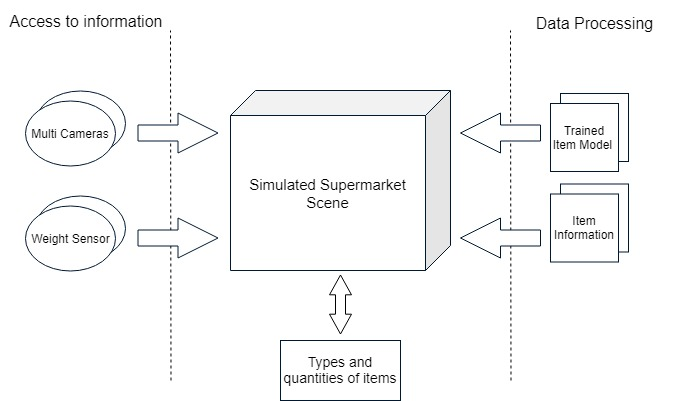
\includegraphics[width=7cm,scale=0.8]{flow.jpg}}
\caption{Architecture of our simulated scenarios}
\label{fig}
\end{figure}

Draw on the company what we talked about earlier, in order to achieve the goal, there are some items we should design first.
This scene includes the size of the shelves, the selection of the camera and the shooting angle and shooting range.
Finally, the recognition system is used to identify the scene.
The model scene is base on a truth supermarket.
In our experiment, we try to achieve this goal and apply it to reality.
Next we will discuss how to build the simulation scenario and the origin of the parameters.


\subsection{Multi cameras and Build scene}

In the previous section, we discussed which recognition system is suitable for shopping mall, most of them are small and medium-sized supermarkets, such as FamilyMart, JOETEN, 7-ELEVEN.
Through a large number of investigations into them, we find that the general pattern of these supermarkets is used strip shelves and parallel emissions.
Strip shelves and parallel emissions which has the advantages of easy placement and customer selection, this is the most common way to put it on the market.
It's also suitable for us to use cameras to observe the whole scene and the shelves, we will also use this placement in scene construction.
And then we draw lessons from their pattern, it can use the Unity3D to achieve the scene.
We used multi cameras in our simulated scenario, and try to restore the real scene as much as possible.
The Multi cameras scene is based on field of view(FOV), the horizontal field of view(H-FOV) and vertical field of view(V-FOV)\cite{Ball88} determined the sharpness and size of the pictures what we get.

\begin{figure}[htbp]
\centerline{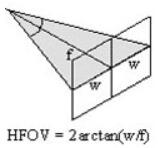
\includegraphics[width=2.5cm,scale=0.4]{HFOV.jpg} 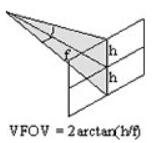
\includegraphics[width=2.5cm,scale=0.4]{VFOV.jpg}}
\caption{H-FOV and V-FOV .}
\label{fig}
\end{figure}

Fixed focal length lens, it can get the angel field of view(AFOV), and we can get different size of FOV through adjusting the focal length of the lens through different working distances.

\centerline{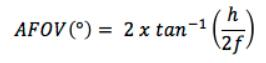
\includegraphics[width=5cm,scale=0.9]{AFOV-MA.jpg}}
\begin{figure}[htbp]
\centerline{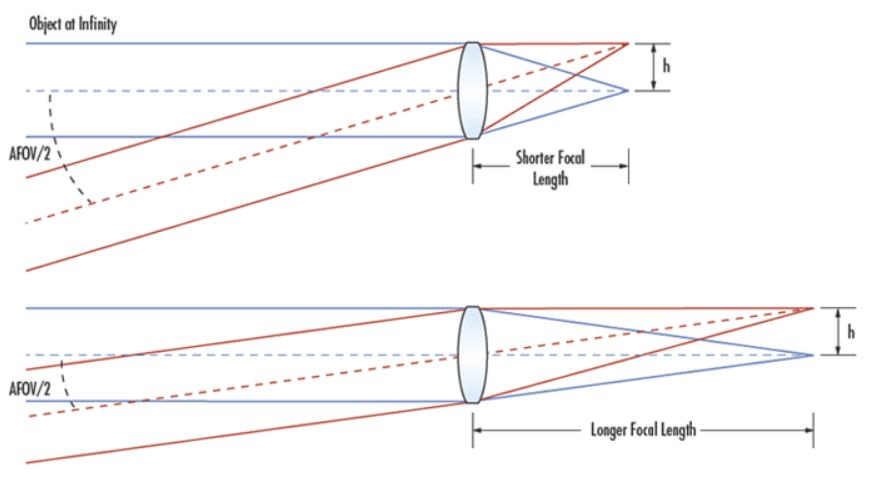
\includegraphics[width=9cm,scale=0.9]{AFOV.jpg}}
\caption{The field of view of lens is related to focal length, f is the focal length, h is the horizontal dimension of the sensor.}
\label{fig}
\end{figure}

We can follow the specifications of the scene (shelves size, the length and width of walking, and layout of the whole scene) to adjust FOV.


\subsection{Cameras Selected}

The terms "dots per inch" (DPI) and "pixels per inch"(PPI) are used interchangeably by many. A 200 dpi print means that for each inch of that printed material, it takes about 200 dots to make the picture. A pixel is like a square dot without gaps. Both of them can describe the quality of a picture, and some cameras save digital images in arbitrary values as 72 dpi. We can calculate the DPI or PPI for what we need page size in Fig.5.

\begin{figure}[htbp]
\centerline{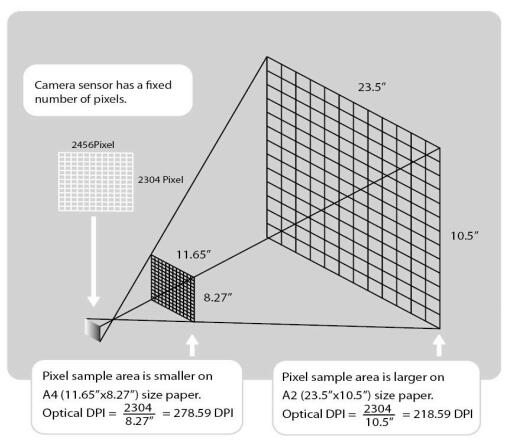
\includegraphics[width=8cm,scale=0.9]{DPIPPI.jpg}}
\caption{DPI and PPI}
\label{fig}
\end{figure}

FLEXIDOME IP panoramic 7000 MP, which has 12MP / 30 fps sensor for fine details with smooth motion and Intelligent Video Analysis on full panoramic overview. Panoramic surveillance offers full 180�� or 360�� coverage of the designated area. The 360�� version of the camera, when mounted
centrally on a ceiling, gives complete wall-to-wall coverage. The 180�� version has a higher effective resolution and is ideal for wall mounting or for ceiling
mounting in corridors.

When mounted at a height of 3.5 m (11.48 ft) the 360�� version of the camera has the following coverage radius for the four levels in Fig.6.

\begin{figure}[htbp]
\centerline{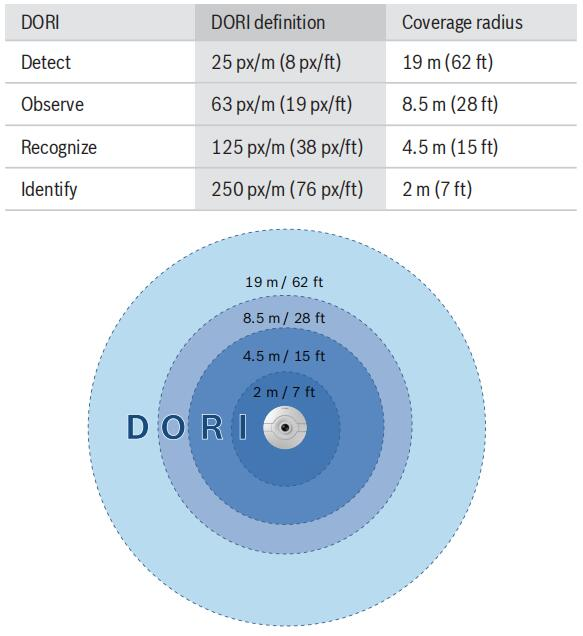
\includegraphics[width=7cm,scale=0.8]{camera360.jpg}}
\caption{Scope of sight of 360�� version camera}
\label{fig}
\end{figure}

When mounted at a height of 3.5 m (11.48 ft) the 180�� version of the camera has the following coverage radius for the four levels in Fig.7.

\begin{figure}[htbp]
\centerline{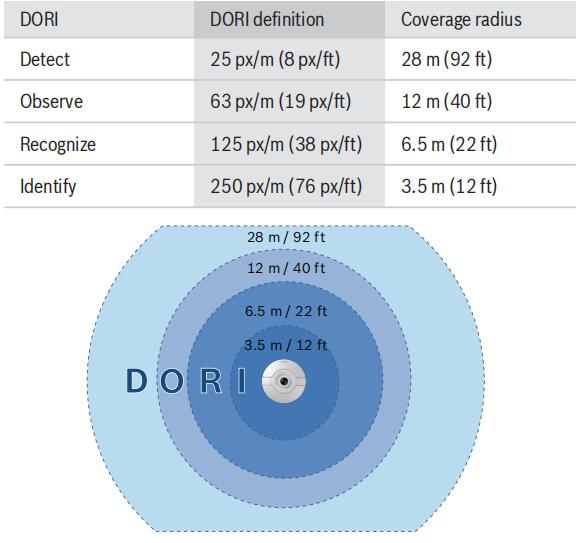
\includegraphics[width=7cm,scale=0.8]{camera180.jpg}}
\caption{Scope of sight of 180�� version camera}
\label{fig}
\end{figure}

The camera provides the full resolution circular image for recording even if we are viewing only a portion of the scene.
Unity3D is a game engine, the engine can be used to create both three-dimensional and two-dimensional games as well as simulations for its many platforms.
In our experiment, we use Unity3D to build a scene like a truth supermarket, and camera placement experiments are performed in this simulated scene.

\subsection{Item Recognition}

The main method current approaches to object recognition make essential use of machine learning methods and deep learning methods.
To achieve the item recognition, we can collect larger datasets, learn more powerful models, and use better techniques for preventing overfitting.
In order to achieve item recognition, we use the YOLOv3 method to train our datasets.
YOLO means "You only look once, real time object detection explained", it is a new item recognition method, now it has developed to the 3rd generation, it has more accurate recognition rate and ability to process larger amounts of data.
We will use the YOLOv3 to train image what we get, it is based on OpenCV3.40 and CUDA8.0.

A single GTX 1060 GPU has 6GB of memory, it is enough for us to train examples, therefore we spread the net across GPU.
We can use the Python Reptile to get image from Internet, then use visual GUI-software for marking bounded boxes of objects and generating annotation files.
It will create .txt-file for each .jpg-image-file in the same directory and with the same name, but with .txt-extension, and put to file: object number and object coordinates on this image, for each object in new line: object-class, x, y, width, height.



\section{Simulator}

In the previous section, we already introduce how to design scenarios and how to arrange them.
After we have explored and designed these necessary parameters.
Then in this section, we start with building up the scenarios described earlier.
It is included achieve the cashier-free supermarket in Unity3D, and the item recognition method what we use, then we combine them into a whole and application of simulation in real scene.

\subsection{Scene simulation}

Achieving our scene in Unity3D  which can simulate scene like a truth supermarket, the model is basic on the layout of Supermarket after our investigation.
It is length and width and height of the scene are 40m, 25m, 6m, and aisle width is 2.7m.
In the scene we set 5 bins, and each of bin width is 2.35m and height is 1.7m.
When have built the scene, we can design add the multi cameras to our scene, then put the cameras on the bins.
In the scene we put the each camera on the bins which height is 2.22m, it is through our calculation, the most conducive to obtaining the height of the image, and set cameras 6.8m apart from the previous calculations.
Then build four-direction cameras on the aisle, which is placed every 3 meters above the corridor, the cameras coverage needs to cover the entire scene.
A four-direction camera has 4 cameras for 4 directions, and we put them on the 3.5m. height of aisle.
In the scene we built, we totaly use 152 cameras in this scene.
The overall layout is shown in the Fig.8.

\begin{figure}[htbp]
\centerline{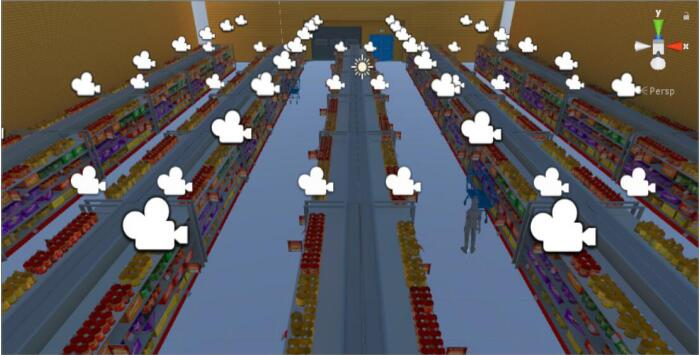
\includegraphics[width=7cm,scale=0.8]{supermarket.jpg}}
\caption{The whole simulated supermarket scene}
\label{fig}
\end{figure}

After setting up the scene, we also need to adjust the visual field and angle of each camera to get the best shooting pictures.
Through calculation and field investigation, we draw the h-fov is 1.2 bin is best for catching the maximum range and clearer picture, and the each camera can cover 2 bin.
In Fig.9, we can see the cameras which on shelves can clearly obtain the type and quantity of items, this provides a great help for our later identification.

\begin{figure}[htbp]
\centerline{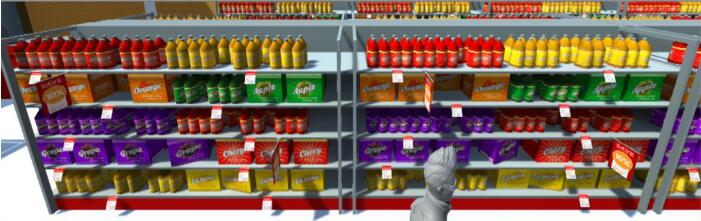
\includegraphics[width=7cm,scale=0.8]{shelves.jpg}}
\caption{Information on the shelf captured by camera shuttle}
\label{fig}
\end{figure}

The simulated scene is based on the real scene, it can serve as a reference.
In this scene, we can design the placement of cameras, and calculate the location of the camera in the real scene and the number of cameras needed.
Unity3D provide method of capturing each camera image, use the clear screenshot F9 to get the picture which is describe the items type and quantity on shelves, and it is resolution is 1600*1200.
Then use pictures what we get to do item recognition and identify their type and number, ultimately get the data for the all items, calculate what kind and quantity customers take away.

\subsection{Item Recognition}

After setting up the scene, we need to add an image recognition system to each camera in the scene.
As mentioned above, YOLOv3 is suitable for items image recognition, we will use this recognition method for items image processing.
The YOLOv3 depends on OpenCV3.40 and CUDA8.0, which are our tools for training and recognition.
There are other ways to train and recognize our data.
TensorFlow\cite{199317} is a free and open-source software library for dataflow and differentiable programming across a range of tasks, it can as well be used in computer vision processing.
In our simulation, OpenCV still is our main train and recognize, because it's easier to operate in our limited equipment.

In order to recognize the picture what we get for the scene's cameras, we have to pre-process the types of items and train them.
There are lots of goods pictures in the internet, then we selected 1000 representative types for us to train.
In order to make the simulation results closer to the real scene, the goods we selected were placed on the shelves and they were placed according to the way of the shopping mall.
After obtaining samples pictures, these pictures should be marked so that the system can remember their characteristics and what exactly item is.

\begin{figure}[htbp]
\centerline{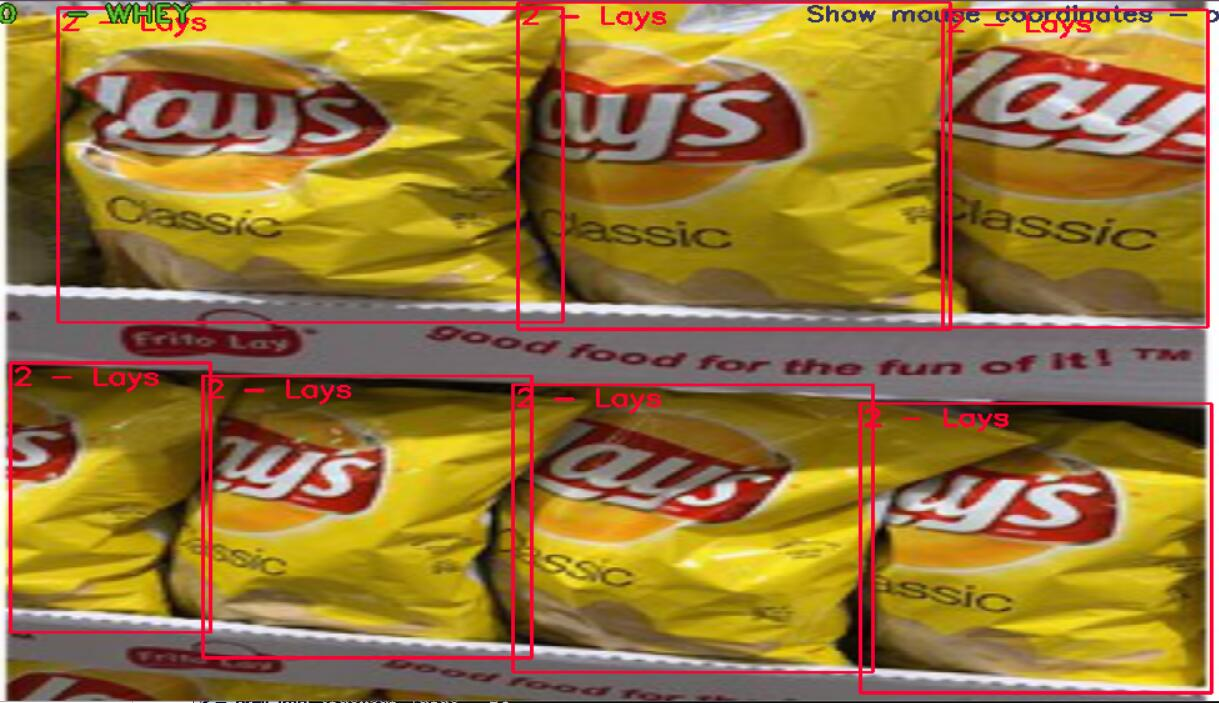
\includegraphics[width=7cm,scale=0.8]{LaysMarked.jpg}}
\caption{The test set image what we use in our experiment}
\label{fig}
\end{figure}

After marking all items, we will put all the pictures and data of the pictures into our pre-designed YOLO architecture for training.
The purpose of training is to get the weight of each item so that our system can distinguish their type and accurately judge when inputting new pictures.
In our simulator, we had 5,000 iterations of the data to get a lowest loss.
When all the data has been trained, new data can be allowed to enter.
We selected a picture that was not included in our data set to try the training results.
The category of this item is the one that has been trained by our system.
We searched the pictures of this item randomly on the Internet and put them into our system for identification.
The recognition result as shown in Fig.11

\begin{figure}[htbp]
\centerline{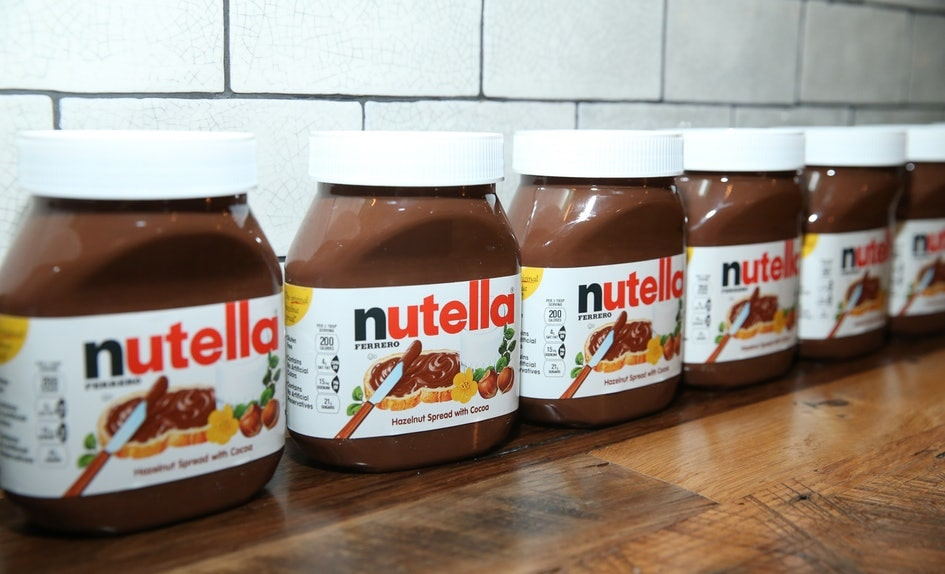
\includegraphics[width=3.5cm,scale=0.6]{nutella.jpg} 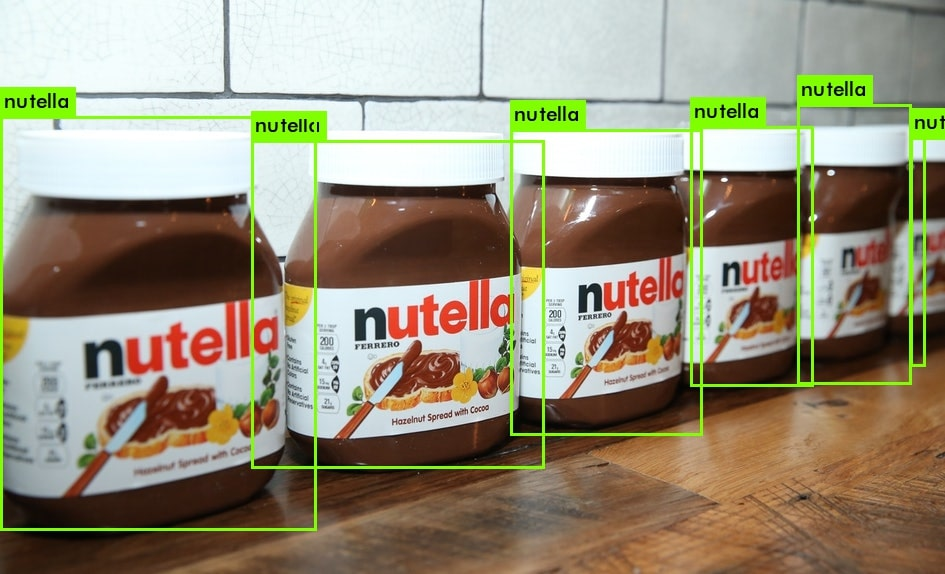
\includegraphics[width=3.5cm,scale=0.6]{nutella2.jpg}}
\caption{Put the "nutella" pictures into our recognition system and recognize the information.}
\label{fig}
\end{figure}

Our system can accurately identify the object and the number of objects in this picture, its recognition rate can reach 98\%.
This means that when the camera in the scene intercepts the picture and puts it into our system, it can accurately identify the type and number of them.
It shows that the system we built is feasible to be used in real scenes.
Ultimately we'll have it with multi cameras to achieve cashier-free supermarket.




As for the experiment, the concept of "cashier-free supermarket" can be achieved by our simulator scene.
And we can make good use of our experimental results in small and medium-sized supermarkets.
By investigating supermarkets on the market, such as 7-11, Family, GIANT.
Most of them can use the multi camera recognition system, and shown in Fig.12

\begin{figure}[htbp]
\centerline{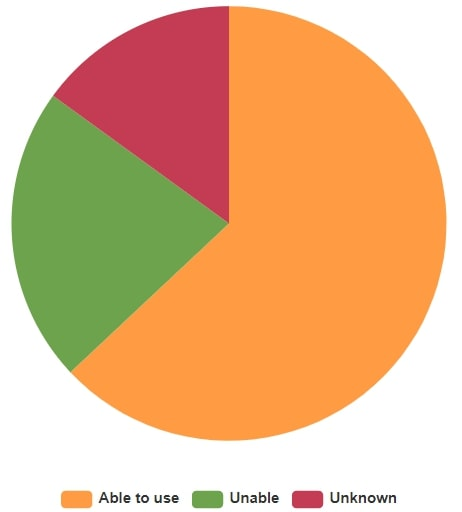
\includegraphics[width=3cm,scale=0.3]{pie.jpg}}
\caption{Through our survey, the supermarkets whether can use our identification system}
\label{fig}
\end{figure}

In the pie chart, 63\% supermarket can use the recognition system directly.
11\% supermarkets may be unavailable due to shelf placement or small area.
According to the survey, most supermarkets can use this recognition system.

However, there are many problems to be solved meanwhile.
When there are too many people in the supermarket, they will interfere with camera shooting.
How to identify two objects with the same weight and very similar weight accurately.
These are the problems we need to solve in the future.


%\begin{table}[htbp]
%\caption{Table Type Styles}
%\begin{center}
%\begin{tabular}{|c|c|c|c|}
%\hline
%\textbf{Table}&\multicolumn{3}{|c|}{\textbf{Table Column Head}} \\
%\cline{2-4}
%\textbf{Head} & \textbf{\textit{Table column subhead}}& \textbf{\textit{Subhead}}& \textbf{\textit{Subhead}} \\
%\hline
%copy& More table copy$^{\mathrm{a}}$& &  \\
%\hline
%\multicolumn{4}{l}{$^{\mathrm{a}}$Sample of a Table footnote.}
%\end{tabular}
%\label{tab1}
%\end{center}
%\end{table}



\bibliographystyle{IEEEtran}
\bibliography{refer_output}


\vspace{12pt}


\end{document}
